\documentclass[
  shownotes,
  xcolor={svgnames},
  hyperref={colorlinks,citecolor=DarkBlue,linkcolor=DarkRed,urlcolor=DarkBlue}
  ]{beamer}
\usepackage{animate}
\usepackage{amsmath}
\usepackage{amsfonts}
\usepackage{amssymb}
\usepackage{pifont}
\usepackage{mathpazo}
%\usepackage{xcolor}
\usepackage{multimedia}
\usepackage{fancybox}
\usepackage[para]{threeparttable}
\usepackage{multirow}
\setcounter{MaxMatrixCols}{30}
\usepackage{subcaption}
\usepackage{graphicx}
\usepackage{lscape}
\usepackage[compatibility=false,font=small]{caption}
\usepackage{booktabs}
\usepackage{ragged2e}
\usepackage{chronosys}
\usepackage{appendixnumberbeamer}
\usepackage{animate}
\setbeamertemplate{caption}[numbered]
\usepackage{color}
%\usepackage{times}
\usepackage{tikz}
\usepackage{comment} %to comment
%% BibTeX settings
\usepackage{natbib}
\bibliographystyle{apalike}
\bibpunct{(}{)}{,}{a}{,}{,}
\setbeamertemplate{bibliography item}{[\theenumiv]}

% Defines columns for bespoke tables
\usepackage{array}
\newcolumntype{L}[1]{>{\raggedright\let\newline\\\arraybackslash\hspace{0pt}}m{#1}}
\newcolumntype{C}[1]{>{\centering\let\newline\\\arraybackslash\hspace{0pt}}m{#1}}
\newcolumntype{R}[1]{>{\raggedleft\let\newline\\\arraybackslash\hspace{0pt}}m{#1}}


\usepackage{xfrac}


\usepackage{multicol}
\setlength{\columnsep}{0.5cm}

% Theme and colors
\usetheme{Boadilla}

% I use steel blue and a custom color palette. This defines it.
\definecolor{andesred}{HTML}{af2433}

% Other options
\providecommand{\U}[1]{\protect\rule{.1in}{.1in}}
\usefonttheme{serif}
\setbeamertemplate{itemize items}[default]
\setbeamertemplate{enumerate items}[square]
\setbeamertemplate{section in toc}[circle]

\makeatletter

\definecolor{mybackground}{HTML}{82CAFA}
\definecolor{myforeground}{HTML}{0000A0}

\setbeamercolor{normal text}{fg=black,bg=white}
\setbeamercolor{alerted text}{fg=red}
\setbeamercolor{example text}{fg=black}

\setbeamercolor{background canvas}{fg=myforeground, bg=white}
\setbeamercolor{background}{fg=myforeground, bg=mybackground}

\setbeamercolor{palette primary}{fg=black, bg=gray!30!white}
\setbeamercolor{palette secondary}{fg=black, bg=gray!20!white}
\setbeamercolor{palette tertiary}{fg=white, bg=andesred}

\setbeamercolor{frametitle}{fg=andesred}
\setbeamercolor{title}{fg=andesred}
\setbeamercolor{block title}{fg=andesred}
\setbeamercolor{itemize item}{fg=andesred}
\setbeamercolor{itemize subitem}{fg=andesred}
\setbeamercolor{itemize subsubitem}{fg=andesred}
\setbeamercolor{enumerate item}{fg=andesred}
\setbeamercolor{item projected}{bg=gray!30!white,fg=andesred}
\setbeamercolor{enumerate subitem}{fg=andesred}
\setbeamercolor{section number projected}{bg=gray!30!white,fg=andesred}
\setbeamercolor{section in toc}{fg=andesred}
\setbeamercolor{caption name}{fg=andesred}
\setbeamercolor{button}{bg=gray!30!white,fg=andesred}


\usepackage{fancyvrb}
\newcommand{\VerbBar}{|}
\newcommand{\VERB}{\Verb[commandchars=\\\{\}]}
\DefineVerbatimEnvironment{Highlighting}{Verbatim}{commandchars=\\\{\}}
% Add ',fontsize=\small' for more characters per line
\usepackage{framed}
\definecolor{shadecolor}{RGB}{248,248,248}
\newenvironment{Shaded}{\begin{snugshade}}{\end{snugshade}}
\newcommand{\AlertTok}[1]{\textcolor[rgb]{0.94,0.16,0.16}{#1}}
\newcommand{\AnnotationTok}[1]{\textcolor[rgb]{0.56,0.35,0.01}{\textbf{\textit{#1}}}}
\newcommand{\AttributeTok}[1]{\textcolor[rgb]{0.77,0.63,0.00}{#1}}
\newcommand{\BaseNTok}[1]{\textcolor[rgb]{0.00,0.00,0.81}{#1}}
\newcommand{\BuiltInTok}[1]{#1}
\newcommand{\CharTok}[1]{\textcolor[rgb]{0.31,0.60,0.02}{#1}}
\newcommand{\CommentTok}[1]{\textcolor[rgb]{0.56,0.35,0.01}{\textit{#1}}}
\newcommand{\CommentVarTok}[1]{\textcolor[rgb]{0.56,0.35,0.01}{\textbf{\textit{#1}}}}
\newcommand{\ConstantTok}[1]{\textcolor[rgb]{0.00,0.00,0.00}{#1}}
\newcommand{\ControlFlowTok}[1]{\textcolor[rgb]{0.13,0.29,0.53}{\textbf{#1}}}
\newcommand{\DataTypeTok}[1]{\textcolor[rgb]{0.13,0.29,0.53}{#1}}
\newcommand{\DecValTok}[1]{\textcolor[rgb]{0.00,0.00,0.81}{#1}}
\newcommand{\DocumentationTok}[1]{\textcolor[rgb]{0.56,0.35,0.01}{\textbf{\textit{#1}}}}
\newcommand{\ErrorTok}[1]{\textcolor[rgb]{0.64,0.00,0.00}{\textbf{#1}}}
\newcommand{\ExtensionTok}[1]{#1}
\newcommand{\FloatTok}[1]{\textcolor[rgb]{0.00,0.00,0.81}{#1}}
\newcommand{\FunctionTok}[1]{\textcolor[rgb]{0.00,0.00,0.00}{#1}}
\newcommand{\ImportTok}[1]{#1}
\newcommand{\InformationTok}[1]{\textcolor[rgb]{0.56,0.35,0.01}{\textbf{\textit{#1}}}}
\newcommand{\KeywordTok}[1]{\textcolor[rgb]{0.13,0.29,0.53}{\textbf{#1}}}
\newcommand{\NormalTok}[1]{#1}
\newcommand{\OperatorTok}[1]{\textcolor[rgb]{0.81,0.36,0.00}{\textbf{#1}}}
\newcommand{\OtherTok}[1]{\textcolor[rgb]{0.56,0.35,0.01}{#1}}
\newcommand{\PreprocessorTok}[1]{\textcolor[rgb]{0.56,0.35,0.01}{\textit{#1}}}
\newcommand{\RegionMarkerTok}[1]{#1}
\newcommand{\SpecialCharTok}[1]{\textcolor[rgb]{0.00,0.00,0.00}{#1}}
\newcommand{\SpecialStringTok}[1]{\textcolor[rgb]{0.31,0.60,0.02}{#1}}
\newcommand{\StringTok}[1]{\textcolor[rgb]{0.31,0.60,0.02}{#1}}
\newcommand{\VariableTok}[1]{\textcolor[rgb]{0.00,0.00,0.00}{#1}}
\newcommand{\VerbatimStringTok}[1]{\textcolor[rgb]{0.31,0.60,0.02}{#1}}
\newcommand{\WarningTok}[1]{\textcolor[rgb]{0.56,0.35,0.01}{\textbf{\textit{#1}}}}
\usepackage{graphicx}
\makeatletter

\makeatother






%%%%%%%%%%%%%%% BEGINS DOCUMENT %%%%%%%%%%%%%%%%%%

\begin{document}

\title[Lecture 4]{Lecture 4: \\ MSE, Prediction Error \\ Github Tools}
\subtitle{Big Data and Machine Learning for Applied Economics \\ Econ 4676}
\date{\today}

\author[Sarmiento-Barbieri]{Ignacio Sarmiento-Barbieri}
\institute[Uniandes]{Universidad de los Andes}


\begin{frame}[noframenumbering]
\maketitle
\end{frame}

%%%%%%%%%%%%%%%%%%%%%%%%%%%%%%%%%%%
%       Motivation              %
% What is the question?
% Why do we care?
% What is new?
% What do you find?
%%%%%%%%%%%%%%%%%%%%%%%%%%%%%%%%%%%




\begin{frame}
\frametitle{Agenda}

\tableofcontents


\end{frame}


%----------------------------------------------------------------------%

\begin{frame}
\frametitle{Recap}

\begin{itemize} 
    \item We started shifting paradigms
    \bigskip
    \item Linear Regression
    \bigskip
    \item Prediction vs Estimation
    \bigskip
    \item Train and Test Samples
    \bigskip
    \item Example in \texttt{R}
\end{itemize}
\end{frame}



%----------------------------------------------------------------------%
\section{Motivation}
%----------------------------------------------------------------------%
\begin{frame}
\frametitle{Motivation}

\begin{itemize}
  \item Working model is
  \begin{align}
  y=f(X)+u
  \end{align}
  \bigskip
  \item Linear regression is the “work horse” of econometrics and (supervised) machine learning. 
  
  \begin{align}
  y=X\beta+u
  \end{align}
  
  
  \begin{itemize}
    \item All the interest is on $\beta$
    \item Gauss-Markov Theorem says that under classical assumptions it is BLUE 
  \end{itemize}
  
\end{itemize}
\end{frame}




%----------------------------------------------------------------------%
\section{Mean Square Error}
%----------------------------------------------------------------------%

\begin{frame}
\frametitle{Mean Square Error}


\begin{align}
  MSE(\beta) &= E(\hat \beta - \beta)^2 \\
             &= E(\beta - E(\hat \beta))^2 + Var(\hat \beta) 
\end{align}

\begin{itemize}
\item  Intuitively, the result says that how wrong is the estimate (MSE) depends on: 
\bigskip
  \begin{itemize}
  \item how uncentered it is (bias) and 
  \item how dispersed it is around its center (variance). 
  \end{itemize}
\end{itemize}



\end{frame}

\begin{frame}
\frametitle{Mean Square Error}

%----------------------------------------------------------------------%

\begin{figure}[H] \centering
  \centering
  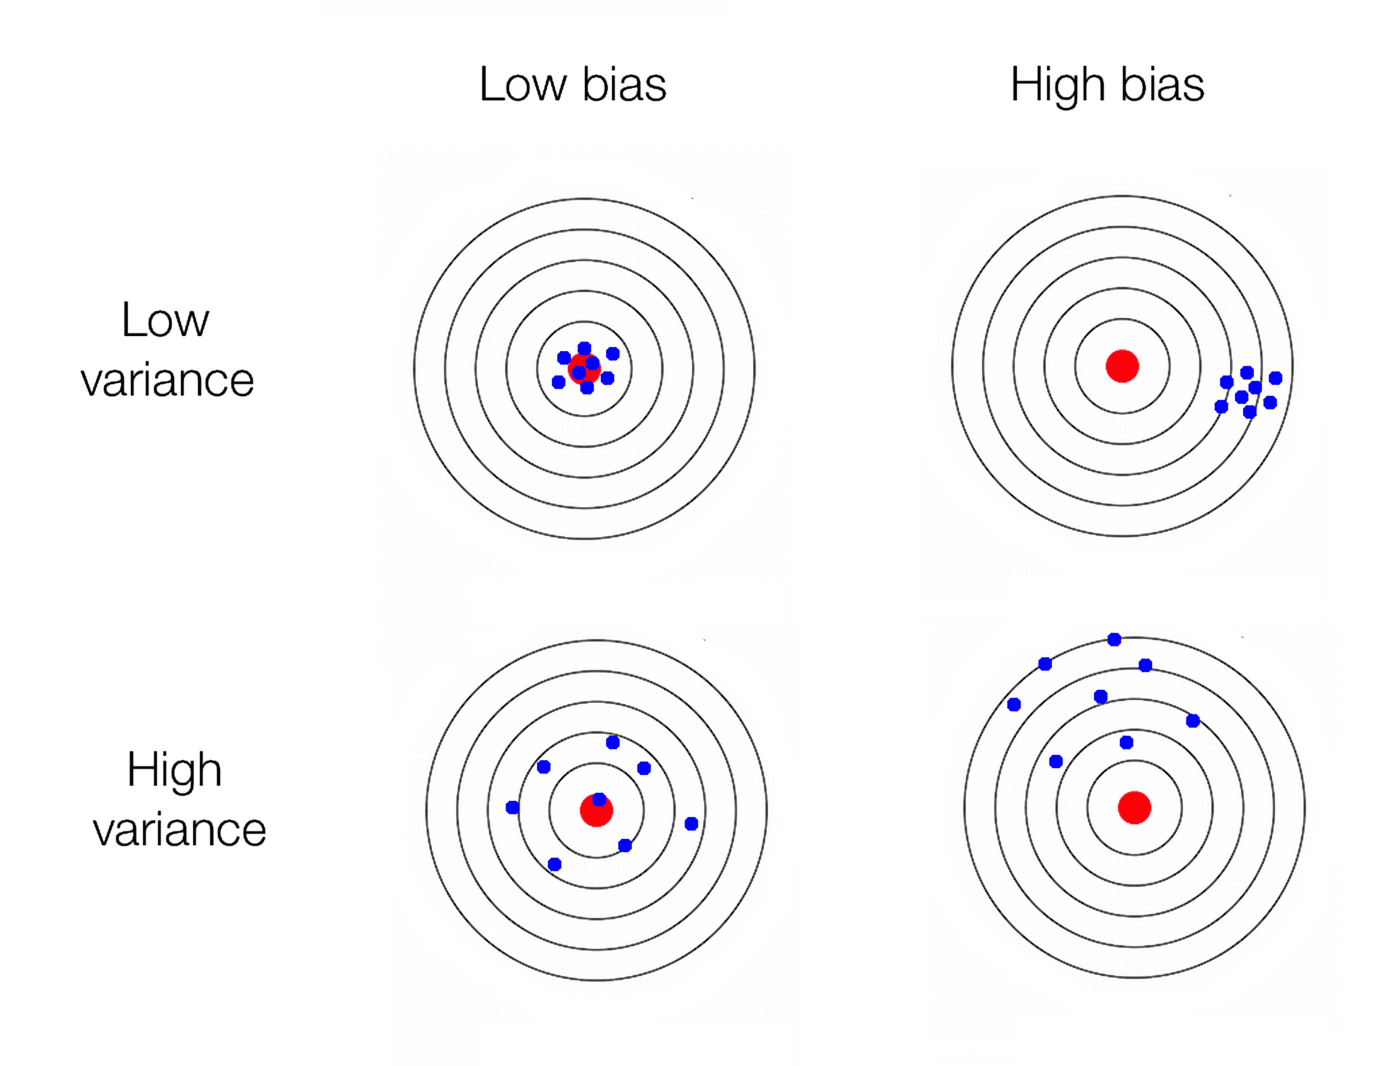
\includegraphics[scale=0.15]{figures/medium_bias_variance.png}
  \\
  \tiny
  Source: https://tinyurl.com/y3xlh87o
\end{figure}


\end{frame}

%----------------------------------------------------------------------%
\section{Prediction Error}
%----------------------------------------------------------------------%

\begin{frame}
\frametitle{Prediction Error}

\begin{itemize}
  \item Now suppose that the goal is to predict $Y$ with another random variable $\hat Y$.
  \bigskip
  \item The \emph{prediction error} is defined as:
\end{itemize}
  \bigskip

  \begin{align}
    Err(\hat Y) \equiv E\left(Y-\hat Y\right)^2\
  \end{align}

\begin{itemize}
  \item Conceptually the prediction error is equal to the MSE
  \bigskip
  \begin{itemize}
  \item MSE compares a RV ($\hat \beta$) with a parameter ($\beta$)
  \bigskip
  \item  $Err(\hat Y)$  involves two RV 
  \end{itemize}
\end{itemize}



\end{frame}

%----------------------------------------------------------------------%

\begin{frame}
\frametitle{Prediction Error}


\bigskip
Then 
\begin{align}
  Err (\hat Y )  &= E(Y-\hat f)^2  \\
                 &= MSE(\hat f) + \sigma^2  \\
                 &= Bias^2(\hat f) + V(\hat f) + \sigma^2
\end{align}
\bigskip
Two parts:
\begin{itemize}
  \item  the error from estimating $f$ with $\hat f$. (\emph{reducible})
  \item  the error from not being able to observe $u$. (\emph{irreducible})
\end{itemize}

\bigskip

This is an important result, predicting $Y$ properly we need a good estimate of $f$.

\end{frame}

%----------------------------------------------------------------------%

\begin{frame}
\frametitle{Prediction Error}

\begin{figure}[H] \centering
  \centering
  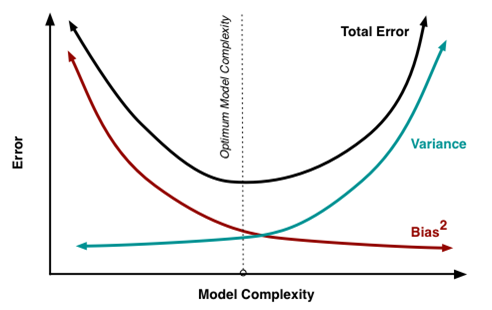
\includegraphics[scale=0.50]{figures/medium_bias_variance_trade_off.png}
  \\
  \tiny
  Source: https://tinyurl.com/y4lvjxpc
\end{figure}


{\tiny A very interesting discussion in a recent Twitter thread by Daniela Witten: \url{https://twitter.com/daniela_witten/status/1292293102103748609?s=20}}
\end{frame}
%----------------------------------------------------------------------%
\begin{frame}
\frametitle{Prediction Error}

\begin{itemize}
  \item Model $y=X\beta +u$
  \item $\hat y=\hat \beta X$ is the prediction 
  \item The estimated prediction error is 
  \begin{align}
    \hat Err (\hat Y ) = \sum (y_i-\hat y_i)^2
  \end{align}

  \item Common alternatives involve: the mean or the square root
  \item In Econometrics 
  \begin{align}
    \hat Err (\hat Y ) = \sum_{i=1}^n e_i^2
  \end{align}
  \item $R^2=1- \frac{Err (\hat Y )}{TSS}$ 
  
  \item OLS minimizes $\hat Err (\hat Y )$ and maximizes $R^2$ $\rightarrow$  minimizing the predictive error is to maximize fit in the sample

  
\end{itemize}
\end{frame}
%----------------------------------------------------------------------%

\begin{frame}
\frametitle{Prediction Error}

\textcolor{red}{Challenge:}

\begin{itemize}
  \item The  goal of machine learning is \emph{out of sample} prediction
  \bigskip
  \item Minimize the prediction error outside of the sample
  \bigskip
  \item OLS designed to minimize inside the sample
  \bigskip
  \item Predicting well in sample doesn't mean that it would work outside
  \bigskip
  \item There are estimators that work very well in sample but very badly outside (Overfit) {\tiny more on this later}
  
\end{itemize}

\end{frame}


%----------------------------------------------------------------------%
\section{Train and Test Samples}
%----------------------------------------------------------------------%
\begin{frame}
\frametitle{Train and Test Samples}


\begin{itemize}
  \item Problem with OLS (and other estimators)
  \medskip
  \begin{itemize}
    \item Minimize the prediction error outside of the sample
    \medskip
    \item OLS designed to minimize inside the sample  
  \end{itemize}
  \bigskip
  
  \item A workaround: split the data
  \medskip
  \begin{itemize}
    \item  Training sample: to build/estimate/train the model
    \medskip
    \item  Test sample:  to evaluate its performance 
  \end{itemize}
\end{itemize}

\end{frame}

%----------------------------------------------------------------------%
\section{ Example: Predicting House Prices in \texttt{R}}
%----------------------------------------------------------------------%
\begin{frame}
\frametitle{Predicting House Prices in \texttt{R}}

\begin{center}
\large Example: Predicting House Prices in \texttt{R} \\
(switch to \texttt{RStudio})
\end{center}


\end{frame}


%----------------------------------------------------------------------%
\section{ Intro to \texttt{Git(Hub)}}
%----------------------------------------------------------------------%
\begin{frame}
\frametitle{ Intro to \texttt{Git(Hub)}}
\framesubtitle{Motivation}

\begin{figure}[H] \centering
  \centering
  
\includegraphics[scale=0.25]{figures/phd101212s}
  \\
  \tiny
  Source: \url{http://phdcomics.com/comics/archive_print.php?comicid=1531}
\end{figure}



\end{frame}
%----------------------------------------------------------------------%

\begin{frame}[fragile]
\frametitle{ Intro to \texttt{Git(Hub)}}
\framesubtitle{Motivation}


\begin{itemize}
\item \texttt{Git}


\begin{itemize}
\medskip
\item Git is a distributed version control system
\medskip
\item It is optimized for the things that economists and data scientists spend a lot of time working
  on (e.g.~code).

\end{itemize}


\bigskip
\item \texttt{GitHub}
\medskip
\begin{itemize}

\item It's important to realize that Git and GitHub are distinct things.
\medskip
\item GitHub is an online hosting platform  built on top of the Git system. (Like Bitbucket and GitLab.)
\medskip
\item Just like we don't \emph{need} Rstudio to run R code, we don't
  \emph{need} GitHub to use Git 
\end{itemize}
\end{itemize}
\end{frame}
%----------------------------------------------------------------------%

\begin{frame}[fragile]
\frametitle{Repositories: Init}

\begin{itemize}
  \item Let's get hands on 
  \bigskip
  \item Create a Repo: go to github and clicking the green ``new repository''

  \begin{itemize}

    \item Step 1: Name your repository 
    \medskip
    \item Step 2: Public or private 
    \medskip
    \item Step 3: Add a README 
    \medskip
    \item Step 4: License e.g. \url{https://choosealicense.com/}
    \medskip
    \item Step 5: gitignore 
  \end{itemize}
    \bigskip
  \item Congratulations!
\end{itemize}
\end{frame}
%----------------------------------------------------------------------%

\begin{frame}[fragile]
\frametitle{Repositories: Clone}



\begin{enumerate}

\item First you need to get your repo url
\bigskip

\item Open up your command line tool, and write \texttt{git\ clone} with the
  url you copied. For example:


\begin{Shaded}
\footnotesize
\begin{Highlighting}[]
\NormalTok{$ }\FunctionTok{git}\NormalTok{ clone https://github.com/ignaciomsarmiento/test\_repo.git}
\end{Highlighting}
\end{Shaded}


\item Go to you click on your file explorer  if you are mousey, type \texttt{ls} (unix based)  or \texttt{dir} (windows) in a terminal window if you are penguinesque.


\begin{Shaded}
\footnotesize
\begin{Highlighting}[]
\NormalTok{$ }\FunctionTok{ls}
\end{Highlighting}
\end{Shaded}


\item  Check what you cloned!
\end{enumerate}
\end{frame}
%----------------------------------------------------------------------%

\begin{frame}[fragile]
\frametitle{Repositories: Useful commands}

\begin{itemize}
  \item See commit history (hit spacebar to scroll down or q to exit).



\begin{Shaded}
\begin{Highlighting}[]
\NormalTok{$ }\FunctionTok{git}\NormalTok{ log}
\end{Highlighting}
\end{Shaded}

\item or what has changed?

\begin{Shaded}
\begin{Highlighting}[]
\NormalTok{$ }\FunctionTok{git}\NormalTok{ status}
\end{Highlighting}
\end{Shaded}

\item to add files

\begin{Shaded}
\begin{Highlighting}[]
\NormalTok{$ }\FunctionTok{git}\NormalTok{ add NAME{-}OF{-}FILE{-}OR{-}FOLDER}
\end{Highlighting}
\end{Shaded}





\end{itemize}

\end{frame}
%----------------------------------------------------------------------%

\begin{frame}[fragile]
\frametitle{Repositories: Useful commands}

You can use \href{https://ryanstutorials.net/linuxtutorial/wildcards.php}{wildcard}
characters to stage a group of files (e.g.~sharing a common prefix).

\begin{itemize}

\item Stage all files.

\begin{Shaded}
\begin{Highlighting}[]
\NormalTok{$ }\FunctionTok{git}\NormalTok{ add {-}A}
\end{Highlighting}
\end{Shaded}



\item Stage updated files only (modified or deleted, but not new).


\begin{Shaded}
\begin{Highlighting}[]
\NormalTok{$ }\FunctionTok{git}\NormalTok{ add {-}u}
\end{Highlighting}
\end{Shaded}



\item  Stage new files only (not updated).

\begin{Shaded}
\begin{Highlighting}[]
\NormalTok{$ }\FunctionTok{git}\NormalTok{ add .}
\end{Highlighting}
\end{Shaded}

  \item Commit your changes.

\begin{Shaded}
\begin{Highlighting}[]
\NormalTok{$ }\FunctionTok{git}\NormalTok{ commit {-}m }\StringTok{"Helpful message"}
\end{Highlighting}
\end{Shaded}

\end{itemize}

\end{frame}
%----------------------------------------------------------------------%

\begin{frame}[fragile]
\frametitle{Repositories: Useful commands}

Pull from the upstream repository (i.e.~GitHub).

\begin{Shaded}
\begin{Highlighting}[]
\NormalTok{$ }\FunctionTok{git}\NormalTok{ pull}
\end{Highlighting}
\end{Shaded}

Push any local changes that you've committed to the upstream repo
(i.e.~GitHub).

\begin{Shaded}
\begin{Highlighting}[]
\NormalTok{$ }\FunctionTok{git}\NormalTok{ push origin master}
\end{Highlighting}
\end{Shaded}

\texttt{origin} is a shorthand name for the remote repository that a
project was originally cloned from. and \texttt{master} the branch we
are pushing to.


\end{frame}


%----------------------------------------------------------------------%

\begin{frame}[fragile]
\frametitle{Collaboration time}

\begin{itemize}
\item I'm going to create "breakout rooms" of two people, and they are going to last 5 min
\medskip
\item This is what I want you to do

  \begin{itemize}

    \item Partner 1: Invite Partner 2 to join you as a collaborator on the \texttt{test\_repo} GitHub repo that you created earlier. (See the \texttt{Settings} tab of your repo.)

    \item Partner 2: Clone Partner 1's repo to your local machine. Make some edits to the README (e.g. delete lines of text and add your own). Stage, commit and push these changes.
    {\tiny Make sure you change into a new directory first, with a different name so you don't have conflicts with your own}

    \item Partner 1: Make your own changes to the README on your local machine. Stage, commit and then try to push them (*after* pulling from the GitHub repo first).

  \end{itemize}


\end{itemize}
\end{frame}
%----------------------------------------------------------------------%

\begin{frame}[fragile]
\frametitle{Collaboration time}
... and we are back
\bigskip
\begin{itemize}
  \item Did Partner 1 encounter a `merge conflict' error? 
  \pause
  \item Check what is going on
  \begin{Shaded}
\begin{Highlighting}[]
\NormalTok{$ }\FunctionTok{git}\NormalTok{status}
\end{Highlighting}
\end{Shaded}


\begin{verbatim}
Unmerged paths:
  (use "git add <file>..." to mark resolution)

   * both modified:   README.md 
\end{verbatim}

\bigskip
\item Git is protecting P1 by refusing the merge. It wants to make sure that you don't accidentally overwrite all of your changes by pulling P2's version of the README.



\end{itemize}
\end{frame}
%----------------------------------------------------------------------%

\begin{frame}[fragile]
\frametitle{Collaboration time}


\begin{verbatim}
# README
Some text here.
<<<<<<< HEAD
Text added by Partner 2.
=======
Text added by Partner 1.
>>>>>>> 814e09178910383c128045ce67a58c9c1df3f558.
More text here.
\end{verbatim}

\end{frame}
%----------------------------------------------------------------------%


\begin{frame}[fragile]
\frametitle{Collaboration time}
\begin{itemize}
  \item Fixing these conflicts is a simple matter of (manually) editing the README file.
  \begin{itemize}
    \item  Delete the lines of the text that you don't want.
    \item  Then, delete the special Git merge conflict symbols.  
  \end{itemize}
  \bigskip
  \item Once that's done, you should be able to stage, commit, pull and finally push your changes to the GitHub repo without any errors.
  \begin{itemize}
    \item P1 gets to decide what to keep because they fixed the merge conflict.
    \item The full commit history is preserved, so P2 can always recover their changes if desired.
    \item Another solution is using \texttt{branches}
  \end{itemize}
\end{itemize}




\end{frame}
%----------------------------------------------------------------------%

\begin{frame}[fragile]
\frametitle{Branches}

\textbf{Incomplete Section in e-TA:} the best pull requests for this section get
some bonus points =)
\begin{itemize}
  \item Branches are one of Git's coolest features.
  \begin{itemize}
    \item Allow you to take a snapshot of your existing repo and try out a whole new idea *without affecting* your main (i.e. "master") branch.
    \item Only once you (and your collaborators) are 100\% satisfied, would you merge it back into the master branch.<sup>1</sup>
    \item This is how most new features in modern software and apps are developed.
    \item It is also how bugs are caught and fixed.
    \item But researchers can easily — and should! — use it to try out new ideas and analysis (e.g. robustness checks, revisions, etc.)
    \item If you aren't happy, then you can just delete the experimental branch and continue as if nothing happened.  
  \end{itemize}


\end{itemize}


\end{frame}
%----------------------------------------------------------------------%

\begin{frame}[fragile]
\frametitle{Branch Shell Commands}

Create a new branch on your local machine and switch to it:
  \begin{Shaded}
\begin{Highlighting}[]
\NormalTok{$ }\FunctionTok{git }\NormalTok{checkout -b NAME-OF-YOUR-NEW-BRANCH}
\end{Highlighting}
\end{Shaded}


Push the new branch to GitHub:
  \begin{Shaded}
\begin{Highlighting}[]
\NormalTok{$ }\FunctionTok{git }\NormalTok{push origin NAME-OF-YOUR-NEW-BRANCH}
\end{Highlighting}
\end{Shaded}


List all branches on your local machine:
  \begin{Shaded}
\begin{Highlighting}[]
\NormalTok{$ }\FunctionTok{git }\NormalTok{branch}
\end{Highlighting}
\end{Shaded}

\end{frame}
%----------------------------------------------------------------------%

\begin{frame}[fragile]
\frametitle{Branch Shell Commands}

Switch back to (e.g.) the master branch:

  \begin{Shaded}
\begin{Highlighting}[]
\NormalTok{$ }\FunctionTok{git }\NormalTok{checkout master}
\end{Highlighting}
\end{Shaded}




Delete a branch
  \begin{Shaded}
\begin{Highlighting}[]
\NormalTok{$ }\FunctionTok{git }\NormalTok{-d NAME-OF-YOUR-FAILED-BRANCH}

\NormalTok{$ }\FunctionTok{git }\NormalTok{push origin :NAME-OF-YOUR-FAILED-BRANCH}
\end{Highlighting}
\end{Shaded}


\end{frame}
%----------------------------------------------------------------------%

\begin{frame}[fragile]
\frametitle{Merging branches + Pull requests}

You have two options:

\begin{enumerate}
\item Locally
\begin{itemize}
  \item Commit your final changes to the new branch (say we call it `new\_idea').
  \item Switch back to the master branch: {\texttt \$ git checkout master}
  \item Merge in the new-idea branch changes: {\texttt \$ git merge new\_idea}
  \item Delete the new-idea branch (optional): {\texttt \$ git branch -d new\_idea}
\end{itemize}



  
  \bigskip
  \item  Remotely (i.e. *pull requests* on GitHub)
  \begin{itemize}

  \item Notify collaborators — or yourself! 
  \item Write a summary of  the changes
  \item You can assign reviewers of your code 
  \end{itemize}



\end{enumerate}



\end{frame}
%----------------------------------------------------------------------%

\begin{frame}[fragile]
\frametitle{Your first pull request}

\begin{itemize}
\item You know that "new\_idea" branch we just created a few slides back? Switch over to it if you haven't already.
\bigskip
\item Remember: 

  \begin{Shaded}
\begin{Highlighting}[]
\NormalTok{$ }\FunctionTok{git}\NormalTok{checkout -b new\_idea}
\end{Highlighting}
\end{Shaded}


\bigskip
\item Make some local changes and then commit + push them to GitHub.
  \medskip
  \begin{itemize}
    \item The changes themselves don't really matter. Add text to the README, add some new files, whatever.
  \end{itemize}

\end{itemize}

\end{frame}
%----------------------------------------------------------------------%

\begin{frame}[fragile]
\frametitle{Your first pull request}

\begin{itemize}

\item After pushing these changes, head over to your repo on GitHub.
\bigskip
  \begin{itemize}
    \item You should see a new green button with "Compare \& pull request". Click it.
    \medskip
    \item Add a meta description of what this PR accomplishes. You can also change the title if you want.
    \medskip
    \item Click "Create pull request".
    \medskip
    \item (Here's where you or your collaborators would review all the changes.)
    \medskip
    \item Once satisfied, click "Merge pull request" and then confirm.
  \end{itemize}

\end{itemize}

\bigskip
For more instructions \url{https://help.github.com/articles/creating-a-pull-request/}

\end{frame}
%----------------------------------------------------------------------%

\begin{frame}[fragile]
\frametitle{Forking}



\begin{itemize}
  \item Forking is going to be the way to contribute to my lectures, e-TAs, etc, and get those precious participation points
\bigskip
\item By forking a repo then you are really creating a copy of it.
\bigskip
\item Once you fork a repo, you are free to do anything you want to it. (It's yours.) 
  \bigskip
\item Combined with a pull request is how you contribute to code development
\end{itemize}



\end{frame}



%----------------------------------------------------------------------%

\begin{frame}
\frametitle{Review \& Next Steps}
  
  \begin{itemize} 
    \item Mean Square Error
    \item Prediction Error
    \item Train and Test Samples
    \item Example in \texttt{R}
    \item Intro to \texttt{Git(Hub)}
  \bigskip  

  
  \item  {\bf Next Class:} Big Data intro, OLS Numerical Properties Computation.
  \bigskip
  \item Questions? Questions about software? 
  
  \end{itemize}


\end{frame}
%----------------------------------------------------------------------%

\section{Further Readings}
%----------------------------------------------------------------------%
\begin{frame}
\frametitle{Further Readings}

\begin{itemize}
  \item Davidson, R., \& MacKinnon, J. G. (2004). Econometric theory and methods (Vol. 5). New York: Oxford University Press.
  \bigskip
  \item James, G., Witten, D., Hastie, T., \& Tibshirani, R. (2013). An introduction to statistical learning (Vol. 112, p. 18). New York: springer.
  \bigskip
  \item Friedman, J., Hastie, T., \& Tibshirani, R. (2001). The elements of statistical learning (Vol. 1, No. 10). New York: Springer series in statistics.
  \bigskip
  \item \texttt{Git} tutorials from \href{https://www.uiuc-bdeep.org/about}{BDEEP group} at \href{http://www.ncsa.illinois.edu/site}{NCSA}. Mimeo.
  \bigskip
  \item \texttt{Git} tutorial from  \href{https://grantmcdermott.com/}{Prof.~Grant McDermott}.


\end{itemize}

\end{frame}


\end{document}


